\documentclass{article}


\usepackage[T1]{fontenc}
\usepackage[short]{optidef}
\usepackage[caption=false,font=footnotesize]{subfig}
\usepackage{adjustbox}
\usepackage{algorithm}
\usepackage{algpseudocode}
\usepackage{amsfonts}
\usepackage{amsmath}
\usepackage{amssymb}
\usepackage{amsthm}
\usepackage{cite}
\usepackage{fullpage}
\usepackage{mathtools}
\usepackage{microtype}
\usepackage{multirow}
\usepackage{pdfpages}
\usepackage{pgfplots}
\usepackage{siunitx}
\usepackage{xr-hyper}
\usepackage{hyperref}

\externaldocument[M-]{submit}

\DeclareSIUnit{\belm}{Bm}
\DeclareSIUnit{\dBm}{\deci\belm}
\DeclareSIUnit{\beli}{Bi}
\DeclareSIUnit{\dBi}{\deci\beli}

\newcounter{reviewer}
\setcounter{reviewer}{0}
\newcounter{point}[reviewer]
\setcounter{point}{0}
\newcounter{response}[reviewer]
\setcounter{response}{0}

\let\svbibcite\bibcite
\def\bibcite#1#2{\svbibcite{#1}{R#2}}
\makeatletter
\let\svbiblabel\@biblabel
\def\@biblabel#1{\svbiblabel{R#1}}
\makeatother

\renewcommand{\theequation}
	{E\arabic{equation}}

\renewcommand{\thefigure}
	{F\arabic{figure}}

\renewcommand{\thetable}
	{T\arabic{table}}

\renewcommand{\thealgorithm}
	{A\arabic{algorithm}}

\newcommand{\reviewer}
	{\stepcounter{reviewer} \bigskip \hrule \section*{Reviewer \thereviewer}}

\renewcommand{\thepoint}
	{\thereviewer.\arabic{point}}

\renewcommand{\theresponse}
	{\thereviewer.\arabic{response}}

\newenvironment{point}
	{\refstepcounter{point} \bigskip \noindent {\textbf{Comment~\thepoint} } ---\ \itshape}
	{\par}

\newenvironment{response}
	{\refstepcounter{response} \medskip \noindent \textbf{Response:}\ }
	{\medskip}


\begin{document}
	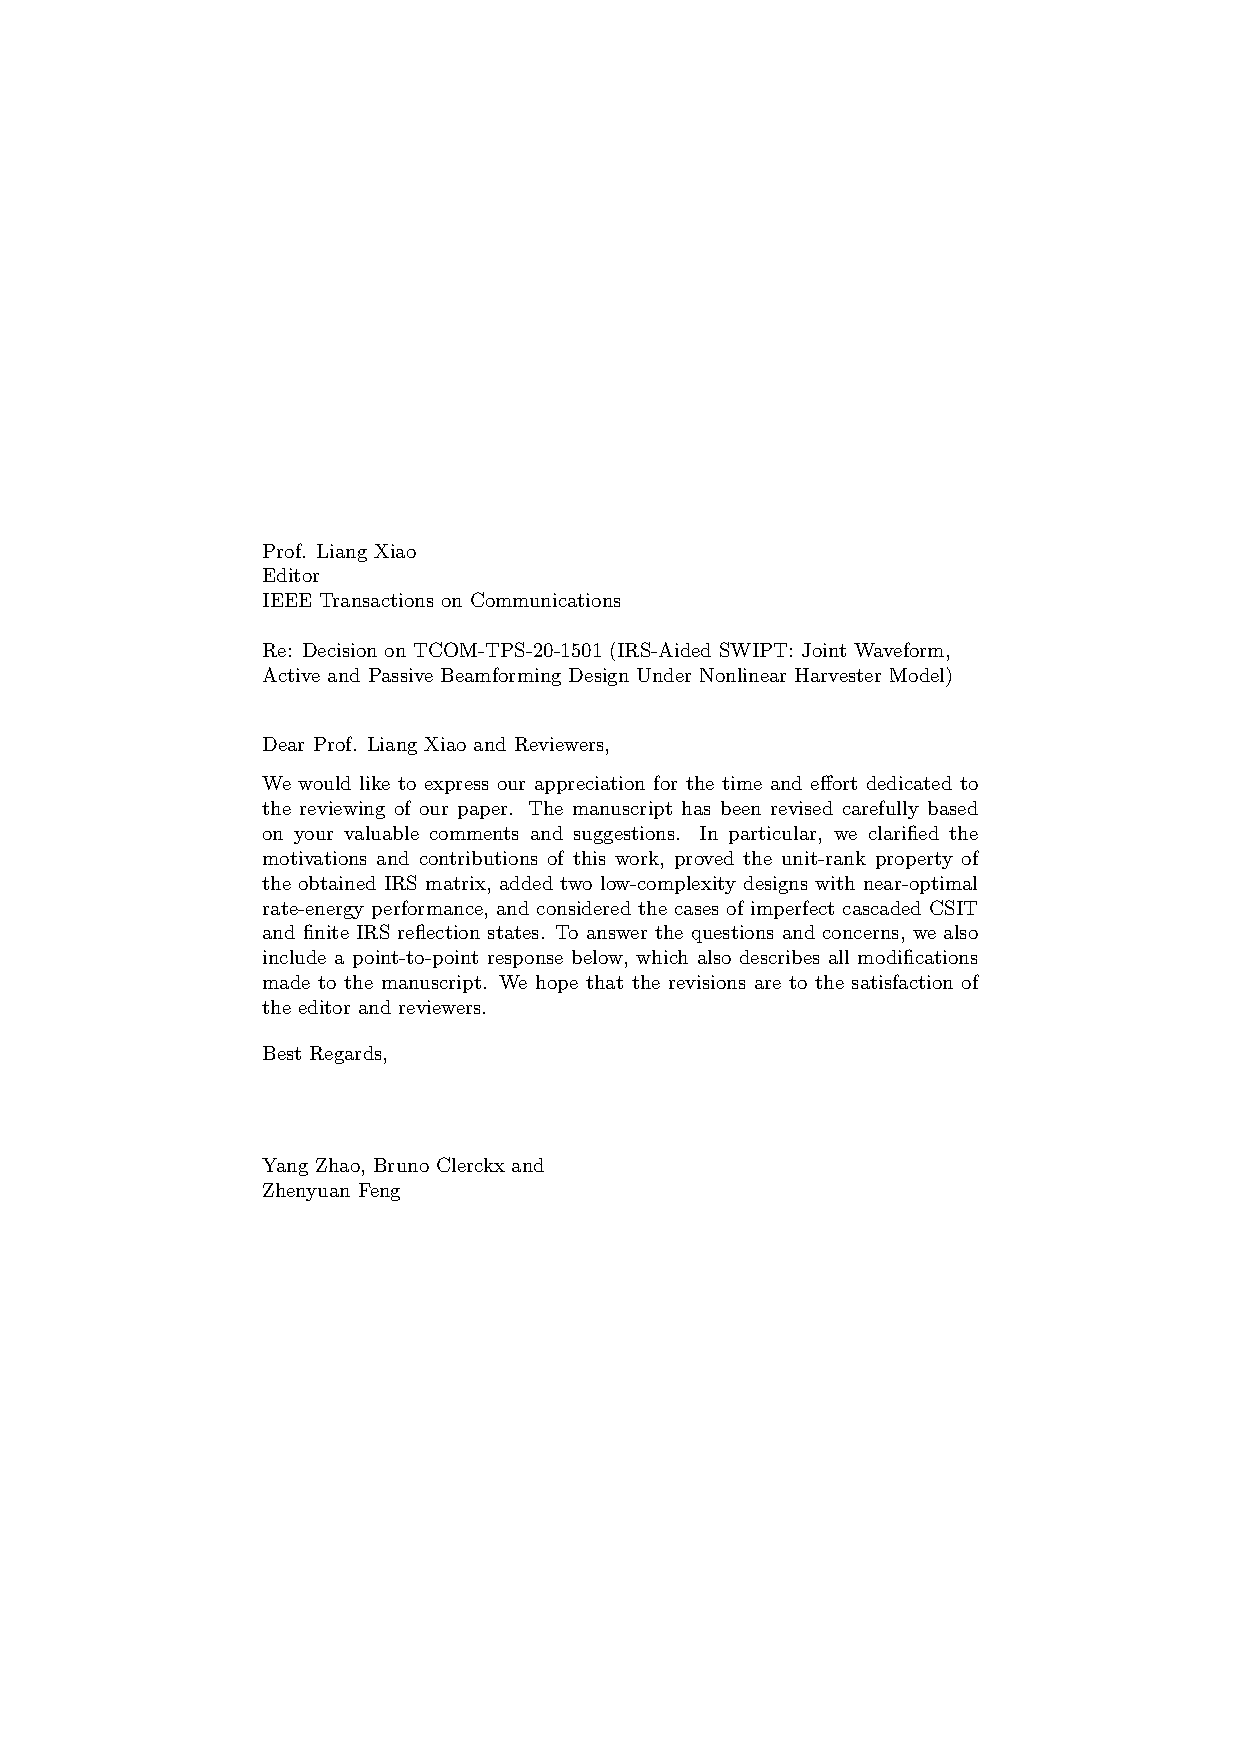
\includepdf{letter_1.pdf}

	\begin{reviewer}
		\begin{point}
			As this paper proposed a BCD-based algorithm and LC-BCD algorithm, it could be better if the authors can further discuss the complexity and provide some measurements or some simulation results.
		\end{point}

		\begin{response}
			TODO
		\end{response}

		\begin{point}
			Since this paper focused on IRS-aided SWIPT systems, it could be better if the authors can further enrich the survey part to make the paper more comprehensive. In particular, some papers have considered this kind of problem from a different aspect such as \cite{Xu2021}. It is kindly suggested to briefly discuss the main difference between \cite{Xu2021} and the problem considered in this paper.
		\end{point}

		\begin{response}
			TODO
		\end{response}

		\begin{point}
			It could be better if the authors can provide some references for the parameter values chosen in the simulation part.
		\end{point}

		\begin{response}
			TODO
		\end{response}

		\begin{point}
			The reviewer noticed that in Algorithm 5, there are two convergence criteria. It could be better if the authors can briefly interpret this issue.
		\end{point}

		\begin{response}
			TODO
		\end{response}
	\end{reviewer}

	\begin{reviewer}
		\begin{point}
			Although this paper reveals many useful insights, most of them are obtained via simulation and then explained via text. The overall theoretical contributions can be greatly improved if the authors can analytically verify or prove some of them, especially those unique to this paper. The authors may conduct the analysis under some simplified or special cases. If some of the observations and findings have been verified in existing papers, the authors can cite and echo these papers wherever necessary.
		\end{point}

		\begin{response}
			TODO
		\end{response}

		\begin{point}
			The authors are suggested to study the impact of IRS passive beamforming on the waveform design without IRS. For example, they can show the optimized waveforms with versus without IRS to unveil the interplay between them. Or even better, analytically compare the two waveforms.
		\end{point}

		\begin{response}
			TODO
		\end{response}

		\begin{point}
			In the introduction, it is suggested to also discuss the new design challenges posed by the nonlinear model compared to the existing designs under the linear model.
		\end{point}

		\begin{response}
			TODO
		\end{response}

		\begin{point}
			In (14), the authors integrated the waveform design and active beamforming design into $\boldsymbol{w}_I$ and $\boldsymbol{w}_P$. However, they separately optimized them later. Is it possible to directly optimize $\boldsymbol{w}_I$ and $\boldsymbol{w}_P$ as a whole?
		\end{point}

		\begin{response}
			TODO
		\end{response}

		\begin{point}
			In the low-complexity BCD, it is unclear how the authors dealt with the optimization of $\rho$ and $\delta$. In Algorithm 5, both of them are input. Did the authors perform a two-dimensional search here? Besides, they were assumed to be identical in the simulation. How will this assumption influence the performance loss?
		\end{point}

		\begin{response}
			TODO
		\end{response}

		\begin{point}
			If possible, in Fig.11, the authors can show the performance of the design under the conventional linear harvester model, so as to show how much performance loss it would incur.
		\end{point}

		\begin{response}
			TODO
		\end{response}

		\begin{point}
			It was shown via simulation that PS is not always superior to TS, unlike the linear model. Is it possible to develop some analytical preconditions to determine which one is better?
		\end{point}

		\begin{response}
			TODO
		\end{response}

		\begin{point}
			Is it possible to give the complexity order of the algorithms presented in this paper?
		\end{point}

		\begin{response}
			TODO
		\end{response}

		\begin{point}
			The expressions of signals in (1), (2), and (5) are not conventional. It may be better to give a per-band signal instead of their superposition. Besides, it is better to first introduce the functionalities of the modulated and multisine waveforms before giving (1).
		\end{point}

		\begin{response}
			TODO
		\end{response}

		\begin{point}
			In Remark 2, the meaning of the sentence, ``there exists a tradeoff for auxiliary link control in the frequency domain'', is not clear to me.
		\end{point}

		\begin{response}
			TODO
		\end{response}

		\begin{point}
			Some editorial comments: 1) ``a (-->an) M-antenna''; 2) ``through a (-->an) L-element IRS''; 3) ``the CSIT of direct and cascaded channels are (-->is) known''; 4) ``It demonstrated (-->demonstrates) that''; 5) In Figs. 9(b) and 10(b), the text in the y-axis is too long. Please divide it into two rows. Besides, the text in the x-axis of the upper figure is covered by the lower one.
		\end{point}

		\begin{response}
			TODO
		\end{response}
	\end{reviewer}

	\begin{reviewer}
		\begin{point}
			Proposition 5 is questionable. The algorithm may not converge to a local optimal due to the coupling constraint 14b.
		\end{point}

		\begin{response}
			TODO
		\end{response}

		\begin{point}
			The figures are too small. For example, Fig 10, the axis legend is not fully shown.
		\end{point}

		\begin{response}
			TODO
		\end{response}

		\begin{point}
			It is said that the reference path loss is -35 dB at 1m, while for the center frequency at 5.18 GHz, even adopting the free space path loss model also will lead a much sever path loss at 1 m. It is not clear how the authors calculate this.
		\end{point}

		\begin{response}
			TODO
		\end{response}

		\begin{point}
			The authors considered the practical reflection coefficient beamforming in the simulkation results. It is not cleaer how the authors obtain the discrte phase shift results. Direct quantization method and some other customized optimization technqiues for discrete phase shifts may have significant performance gap, see \cite{Wu2020c}. Also, this work adopts the same uniform quantization as the above work, which thus needs to be clarified in the paper.
		\end{point}

		\begin{response}
			TODO
		\end{response}

		\begin{point}
			There are also some other practical phase shift models and nonlinear energy harvesting models such as saturation model for IRS-aided SWIPT in existing works, which may be discussed as related works such as amplitude-dependent phase shift model.
		\end{point}

		\begin{response}
			TODO
		\end{response}

		\begin{point}
			Some early magazine papers and recent tutorial papers related to IRS-aided WPT/WIT may be further discussed.
		\end{point}

		\begin{response}
			TODO
		\end{response}
	\end{reviewer}

	\begin{reviewer}
		\begin{point}
			What is the computational complexity of the proposed algorithm?
		\end{point}

		\begin{response}
			TODO
		\end{response}

		\begin{point}
			Some related works are worth citing, such as \cite{Yang2021}.
		\end{point}

		\begin{response}
			TODO
		\end{response}
	\end{reviewer}

	\bibliographystyle{IEEEtran}
	\bibliography{IEEEabrv,library.bib}
\end{document}
